\begin{figure}
  \centering
\definecolor{LightColor}{rgb}{1.0,0.901,0.805}
 
  \definecolor{tile0}{HTML}{DABDE4}
  \definecolor{tile1}{HTML}{B8DBF4}
  \definecolor{tile2}{HTML}{B5EDCD}
  \definecolor{tile3}{HTML}{FBEBA7}
  \definecolor{tile4}{HTML}{F9C1BB}
 
 % Colours
 % --------------------------------------------------------------------------
 % Blue
 
  \definecolor{pastel_0}{HTML}{B8DBF4}
  \definecolor{pastel_1}{HTML}{C1F5FF}
 
 % Purple
 \definecolor{pastel_2}{HTML}{DABDE4}
 \definecolor{pastel_3}{HTML}{BA95C8}
 
 % Red
 \definecolor{pastel_4}{HTML}{F7898F}
 \definecolor{pastel_5}{HTML}{F9C1BB}
 
 % Orange
 \definecolor{pastel_6}{HTML}{FCB68C}
 \definecolor{pastel_7}{HTML}{E5C2A9}
 
 % Yellow
 \definecolor{pastel_8}{HTML}{FFF08A}
 \definecolor{pastel_9}{HTML}{FBEBA7}
 
 % Green
 \definecolor{pastel_10}{HTML}{B5EDCD}
 \definecolor{pastel_11}{HTML}{B3E396}
 
%\def \width-element {\textwidth * 0.2}
%\def \width-buffer {\textwidth * 0.1}
 
%\def \width-grid-element {\width-element * 0.4}
%\def \width-array-element {\width-grid-element * 0.5}
%\newcommand{\wae}{\width-element * 0.2}
 
% width sizes
% Sleutelbuffer = \textwidth * 0.4
%  biffers = \textwidth * 0.2
% Negative space = \textwidth * 0.1
%
% array_element = \textwidth * 0.04 *
% grid_element = \textwidth * 0.08
 
  \tikzstyle{array_element}=[rectangle,
                             minimum size=\textwidth * 0.04,
                             draw=black,
                             rounded corners=2.5, ]
  \tikzstyle{grid_element}=[rectangle,
                            minimum size = \textwidth * 0.08,
                            draw=black,
                            rounded corners=2.5, ]
 
 
  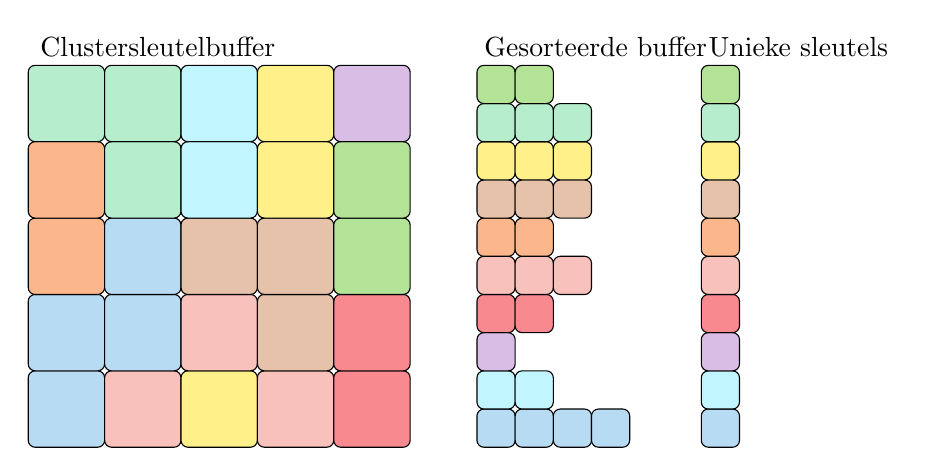
\begin{tikzpicture}
  % Keybuffer
  % -------------------------------------------------------------
  \foreach \i/\c in {0/0, 1/5, 2/8, 3/5, 4/4} {
      \node at (\textwidth * 0.08 * \i, 0) (pixel_\i) [grid_element, fill={pastel_\c}] {};
    }
  \foreach \i/\c in {0/0, 1/0, 2/5, 3/7, 4/4} {
      \node at (\textwidth * 0.08 * \i, \textwidth * 0.08 * 1) (pixel_\i) [grid_element, fill={pastel_\c}] {};
    }
      \foreach \i/\c in {0/6, 1/0, 2/7, 3/7, 4/11} {
      \node at (\textwidth * 0.08 * \i, \textwidth * 0.08 * 2) (pixel_\i) [grid_element, fill={pastel_\c}] {};
    }
      \foreach \i/\c in {0/6, 1/10, 2/1, 3/8, 4/11} {
      \node at (\textwidth * 0.08 * \i, \textwidth * 0.08 * 3) (pixel_\i) [grid_element, fill={pastel_\c}] {};
    }
      \foreach \i/\c in {0/10, 1/10, 2/1, 3/8, 4/2} {
      \node at (\textwidth * 0.08 * \i, \textwidth * 0.08 * 4) (pixel_\i) [grid_element, fill={pastel_\c}] {};
    }
   
    % Sorted buffer
    % -------------------------------------------------------------
    \foreach \i in {0, 1, 2, 3} {
          \node at (\textwidth * 0.45 + \textwidth * 0.04 * \i, \textwidth * 0.04 * 0  -\textwidth * 0.02 ) (pixel_\i) [array_element, fill={pastel_0}] {};
    }
    \foreach \i in {0, 1} {
          \node at (\textwidth * 0.45 + \textwidth * 0.04 * \i, \textwidth * 0.04 * 1  -\textwidth * 0.02 ) (pixel_\i) [array_element, fill={pastel_1}] {};
    }
    \foreach \i in {0} {
          \node at (\textwidth * 0.45 + \textwidth * 0.04 * \i, \textwidth * 0.04 * 2  -\textwidth * 0.02 ) (pixel_\i) [array_element, fill={pastel_2}] {};
    }
    \foreach \i in {0, 1} {
          \node at (\textwidth * 0.45 + \textwidth * 0.04 * \i, \textwidth * 0.04 * 3  -\textwidth * 0.02 ) (pixel_\i) [array_element, fill={pastel_4}] {};
    }
    \foreach \i in {0, 1, 2} {
          \node at (\textwidth * 0.45 + \textwidth * 0.04 * \i, \textwidth * 0.04 * 4  -\textwidth * 0.02 ) (pixel_\i) [array_element, fill={pastel_5}] {};
    }
    \foreach \i in {0, 1} {
          \node at (\textwidth * 0.45 + \textwidth * 0.04 * \i, \textwidth * 0.04 * 5  -\textwidth * 0.02 ) (pixel_\i) [array_element, fill={pastel_6}] {};
    }
    \foreach \i in {0, 1, 2} {
          \node at (\textwidth * 0.45 + \textwidth * 0.04 * \i, \textwidth * 0.04 * 6  -\textwidth * 0.02 ) (pixel_\i) [array_element, fill={pastel_7}] {};
    }
    \foreach \i in {0, 1, 2} {
          \node at (\textwidth * 0.45 + \textwidth * 0.04 * \i, \textwidth * 0.04 * 7  -\textwidth * 0.02 ) (pixel_\i) [array_element, fill={pastel_8}] {};
    }
    \foreach \i in {0, 1, 2} {
          \node at (\textwidth * 0.45 + \textwidth * 0.04 * \i, \textwidth * 0.04 * 8  -\textwidth * 0.02 ) (pixel_\i) [array_element, fill={pastel_10}] {};
    }
    \foreach \i in {0, 1} {
          \node at (\textwidth * 0.45 + \textwidth * 0.04 * \i, \textwidth * 0.04 * 9  -\textwidth * 0.02 ) (pixel_\i) [array_element, fill={pastel_11}] {};
    }
   
    \foreach \i/\c in {0/0, 1/1, 2/2, 3/4, 4/5, 5/6, 6/7, 7/8, 8/10, 9/11} {
          \node at (\textwidth * 0.525 + \textwidth * 0.04 * 4, \textwidth * 0.04 * \i  -\textwidth * 0.02) (pixel_\i) [array_element, fill={pastel_\c}] {};
    }
   
    \node at (-\textwidth * 0.0375, \textwidth * 0.08 * 5) (keybuffer) [anchor=north west] {Clustersleutelbuffer};
    \node at (-\textwidth * 0.0225 + \textwidth * 0.45, \textwidth * 0.08 * 5) (keybuffer) [anchor=north west] {Gesorteerde buffer};
    \node at (\textwidth * 0.04 * 4 + \textwidth * 0.525 -\textwidth * 0.0225, \textwidth * 0.08 * 5) (keybuffer) [anchor=north west] {Unieke sleutels};
  \end{tikzpicture}
  \caption{De sorteer en comprimeer stap uitgevoerd over een enkel vlak.}
  \label{fig:cs-sort-and-compact}
\end{figure}
